%File principale del documento su cui invocare la compilazione, vedi "istruzioni.txt" per più info

%Preambolo: la parte prima del \begin{document}
\documentclass[12pt,a4paper]{article} %formato del documento e grandezza caratteri

%Input del file metadata.tex della cartella locale "res/"
%lista di comandi presenti in template_latex.tex, da qui posso essere modificati secondo le esigenze

\newcommand{\DocTitle}{Verbale interno 2019-11-18} %variabile usata dal file template_latex.tex per settare il titolo del documento
%\newcommand{\DocAuthor}{Progetto "Predire in Grafana"} %variabile usata dal file template_latex.tex per settare l'autore del documento
\newcommand{\DocDate}{18 Novembre 2019} %variabile usata dal file template_latex.tex; Impostata manualmente, altrimenti ad ogni compilazione viene messa la data del giorno di compilazione.
\newcommand{\DocDesc}{Resoconto dell'incontro del gruppo \textit{VRAM Software} tenutosi in data 2019-11-18} %variabile usata dal file template_latex.tex per settare la descrizione del documento
\newcommand{\ver}{27.0.0} %variabile usata dal file template_latex.tex per settare la versione del documento
\newcommand{\app}{Toffoletto Massimo} %variabile usata dal file template_latex.tex per settare l'approvatore del documento
\newcommand{\red}{Dalla Libera Marco} %variabile usata dal file template_latex.tex per settare il redattore del documento
\newcommand{\test}{Schiavon Rebecca} %variabile usata dal file template_latex.tex per settare il verificatore del documento
\newcommand{\stat}{Approvato} %variabile usata dal file template_latex.tex per settare lo stato del documento
\newcommand{\use}{Interno} %variabile usata dal file template_latex.tex per indicare l'uso del documento %Contiene le varibili che descrivono il documento

%Input di file di configurazione presi dalla cartella "Template-LaTeX/config/", uguali per tutti i documenti
%Attenzione bisogna impostare il percorso del file!
% Tutti i pacchetti usati, da inserire nel preambolo prima delle configurazioni

\usepackage[T1]{fontenc} %Permette la sillabazione su qualsiasi testo contenente caratteri
\usepackage[utf8]{inputenc} %Serve per usare la codifica utf-8
\usepackage[english,italian]{babel} %Imposta italiano lingua principale, inglese secondaria. Es. serve per far apparire "indice" al posto di "contents"

\usepackage{graphicx} %Serve per includere le immagini

\usepackage[hypertexnames=false]{hyperref} %Gestisce i riferimenti/link. Es. Serve per rendere clickabili le sezioni dell'indice

\usepackage{float} %Serve per migliore la definizione di oggetti fluttuanti come figure e tabelle. Es. poter usare l'opzione [H] nelle figure ovvero tenere fissate le immagini che altrimenti LaTeX si sposta a piacere.

\usepackage{listings} %Serve per poter mettere snippets di codice nel testo

\usepackage{lastpage} %Serve per poter introdurre un'etichetta a cui si può fare riferimento Es. piè di pagina; poter fare " \rfoot{\thepage\ di \pageref{LastPage}} "

\usepackage{fancyhdr} %Per header e piè di pagina personalizzati

%Sono alcuni package che potranno esserci utili in futuro
%\usepackage{charter}
%\usepackage{eurosym}
\usepackage{subcaption}
%\usepackage{wrapfig}
%\usepackage{background}
\usepackage{longtable} % tabella che può continuare per più di una pagina
\usepackage[table]{xcolor} % ho dovuto aggiungere table in modo da poter colorare le row della tabella, dava: undefined control sequences
%\usepackage{colortbl}

\usepackage{dirtree} % usato per creare strutte tree-view in stile filesystem
\usepackage{xspace} % usato per inserire caratteri spazio
\usepackage[official]{eurosym}
\usepackage{pdflscape} %Inclusione pacchetti
% Configurazioni varie, da inserire nel preambolo dopo i pacchetti

\hypersetup{hidelinks} %serve per nascondere riquadri rossi che circondano i link 

\lstset{literate= {à}{{\`a}}1 } %Permette di usare lettere accentate nei listings

\pagestyle{fancy} %Imposto stile pagina
\fancyhf{} %Reset, se lo tolgo LaTex mette impostazioni di default (p.es numerazione pagine di default)


\lhead{
\includegraphics[scale=0.25]{img/logo_header.png}} %Left header che compare in ogni pagina
%\rhead{\leftmark} %Nome della top-level structure (p.es. Section in article o Chapter in book) in ogni pagina
\rhead{\DocTitle\ v. \ver} %Right header

\newcommand{\glo}{$_G$} %Comando per aggiungere il pedice G
\newcommand{\glosp}{$_G$ } %Comando per aggiungere il pedice G con spazio

\newcommand\Tstrut{\rule{0pt}{2.6ex}} % top padding
\newcommand\Bstrut{\rule[-0.9ex]{0pt}{0pt}} % bottom padding
\newcommand{\TBstrut}{\Tstrut\Bstrut} % top & bottom padding

%Setto il colore dei link
%\hypersetup{
%	colorlinks,
%	linkcolor=[HTML]{404040},
%	citecolor={purple!50!black},
%	urlcolor={blue!50!black}
%}

%Tabelle e tabulazione (può tornare utile)
%\setlength{\tablcolsep}{10pt}
%\renewcommand{\arraystretch}{1.4}

%Comando per aggiungere le pagine di ogni sezione
%\newcommand{\newSection}[1]{%
%	\input{res/sections/#1}
%}

% Comandi per aggiungere padding a parole contenute nella tabella; è una specie di strut (un carattere invisibile)
%\newcommand\Tstrut{\rule{0pt}{2.6ex}} % top padding
%\newcommand\Bstrut{\rule[-0.9ex]{0pt}{0pt}} % bottom padding
%\newcommand{\TBstrut}{\Tstrut\Bstrut} % top & bottom padding  %Configurazione pacchetti

\begin{document}
	%Input del file "frontmatter" preso dalla cartella "Template-LaTeX/config/", uguale per tutti i documenti
	%Attenzione bisogna impostare il percorso del file!
	% #### FRONTESPIZIO (frontmatter) ####
\setlength{\headheight}{33pt} %Distanzia l'header
\pagenumbering{gobble} %Toglie il numero di pagina
\begin{titlepage}
	\begin{center}
		
\includegraphics[scale=0.6]{img/logo.png} \\ %Logo
		\vspace{0.4cm} %Aggiunge uno spazio verticale di 0.5 cm
		
		{\LARGE Progetto "Predire in Grafana"} \\ %Nome progetto
		\vspace{0.4cm} %Attenzione a mettere il punto e NON la virgola
		
		{\Huge \textbf{\DocTitle}} \\ %Titolo, prende variabile definita in metadata.tex
		\vspace{0.4cm}
		
		\DocDate \\ %Data, prende variabile definita in metadata.tex
		\vspace{0.4cm}
		
		%Allineamento colonne: l=left r=right c=center, 
		%va specificato per ogni colonna
		%Se si vuole la riga tra colonne mettere "|"
		
		\begin{tabular}{r | l} %Elementi colonne separate da "&", le righe finiscono con "\\"
			Versione             & \ver \\
			Approvazione         & \app \\ 
			Redazione            & \red \\
			Verifica             & \test \\
			Stato                & \stat \\
			Uso                  & \use \\
		    Destinato a          & Zucchetti \\
						         & Prof. Vardanega Tullio\\
						         & Prof. Cardin Riccardo\\
			Email di riferimento & vram.software@gmail.com
		\end{tabular}
		\vfill
		\textbf{Descrizione} \\
		\DocDesc
	\end{center}
\end{titlepage}
\clearpage

% #### Impostazione header, footer  e numerazione pagine ####
\pagenumbering{arabic} %Pagine con i numeri arabi + reset a 1
\renewcommand{\footrulewidth}{0.4pt} %Di default footrulewidth==0 e quindi è invisibile, di default \headrulewith==0.4pt
\rfoot{\thepage\ di \pageref{LastPage}} %Pagina n di m, con numeri Arabi; usa il pacchetto "lastpage", in caso non sia possibile usare tale pacchetto mettere al fondo dell'ultima pagina "\label{LastPage}"

% #### Tabella dei log ####
% \textbf = grassetto; \Large = font più grande
% \rowcolors{quanti colori alternare}{colore numero riga pari}{colore numero riga dispari}: colori alternati per riga
% \rowcolor{color}: cambia colore di una riga
% p{larghezza colonna}: p è un tipo di colonna di testo verticalmente allineata sopra, ci sarebbe anche m che è centrata a metà ma non è precisa per questo utilizzo TBStrut; la sintassi >{\centering} indica che il contenuto della colonna dovrà essere centrato
% \TBstrut fa parte di alcuni comandi che ho inserito in config.tex che permetto di aggiungere un po' di padding al testo
% \\ [2mm] : questra scrittura indica che lo spazio dopo una break line deve essere di 2mm
% 

%\setcounter{secnumdepth}{0}
%\hfill \break
%\textbf{\Large{Diario delle modifiche}} \\


\addtocontents{toc}{\protect\setcounter{tocdepth}{0}} %Inserire questo per escludere una sezione dall'indice.

\section*{Registro delle modifiche} %Asterisco per fare sezione non numerata
\rowcolors{2}{gray!25}{gray!15}
\begin{longtable} {
		>{\centering}p{17mm} 
		>{\centering}p{19.5mm}
		>{\centering}p{24mm} 
		>{\centering}p{24mm} 
		>{}p{32mm}}
	\rowcolor{gray!50}
	\textbf{Versione} & \textbf{Data} & \textbf{Nominativo} & \textbf{Ruolo} & \textbf{Descrizione} \TBstrut \\
	14.7.0 & 2020-04-09 & Stantagiuliana Vittorio, Toffoletto Massimo e Spreafico Alessandro & \textit{Progettista}, \textit{Verificatore} e \textit{Responsabile di progetto} & Stesura, verifica e approvazione documento. \TBstrut \\ [2mm]
\end{longtable}

\addtocontents{toc}{\protect\setcounter{tocdepth}{4}} %Inserire questo per ripristinare il normale inserimento delle sezioni nell'indice. 4 significa fino al paragrah
\clearpage

% #### INDICE (tableofcontents) ####
\tableofcontents %Provoca la stampa dell'indice
\clearpage

\setcounter{secnumdepth}{4} %Permette di andare fino alla profondità del paragraph con la numerazione delle sezioni %Imposta il frontespizio, l'indice, header e footer
	
	
	
	%Tutte le sezioni del documento
	%\input{res/inserire nome sezione 1} 
	% ...
	%\input{res/inserire nome sezione n} 
	\section{Preventivo} %Meccanismi di controllo e rendicontazione
per ogni fase creare un prospetto delle ore secondo i ruoli ed economico. Per ognuno di essi anche uno riassuntivo.

Viene in seguito presentato il preventivo del costo del lavoro da svolgere con i dettagli sul costo di ogni singolo periodo.
Per identificare i diversi ruoli verranno utilizzate le sigle:
\begin{itemize}
	\item \textbf{Re}: responsabile di progetto;
	\item \textbf{Am}: amministratore di progetto;
	\item \textbf{An}: analista;
	\item \textbf{Pt}: progettista;
	\item \textbf{Pr}: programmatore;
	\item \textbf{Ve}: verificatore;
\end{itemize}
	\subsection{Periodo di analisi}
	Le ore indicate per questo periodo vengono riportate solo perché utili ai fini del documento, non saranno rendicontate nel budget finale richiesto in quanto il periodo di analisi è da considerare come investimento per il gruppo.
		\subsubsection{Prospetto orario}
		Nel periodo di analisi è prevista la seguente divisione oraria:
		\begin{longtable} {				
				>{}p{40mm}  
				>{}p{8mm}
				>{}p{8mm}
				>{}p{8mm}
				>{}p{8mm}
				>{}p{8mm}
				>{}p{8mm}
				>{}p{12mm}				
			}			
			\rowcolor{gray!50}
			\textbf{Nominativo} & \textbf{Re} & \textbf{Am} & \textbf{An} & \textbf{Pt} & \textbf{Pr} & \textbf{Ve} & \textbf{Totale}	\TBstrut \\ [2mm]
			Corrizzato Vittorio & 6 & 6 & 8 & - & - & 5 & 25 \TBstrut \\ [2mm]
			Dalla Libera Marco & 6 & - & 9 & 5 & - & 5 & 25 \TBstrut \\ [2mm]
			Rampazzo Marco & - & 8 & 12 & - & - & 5 & 25 \TBstrut \\ [2mm]
			Santagiuliana Vittorio & - & 5 & 12 & - & - & 8 & 25 \TBstrut \\ [2mm]
			Schiavon Rebecca & - & - & 13 & 5 & - & 7 & 25 \TBstrut \\ [2mm]
			Spreafico Alessandro & - & - & 12 & 5 & - & 8 & 25 \TBstrut \\ [2mm]
			Toffoletto Massimo & 8 & 7 & 5 & - & - & 5 & 25 \TBstrut \\ [2mm]
		\end{longtable}
		Rappresentata nel seguente grafico: \\
		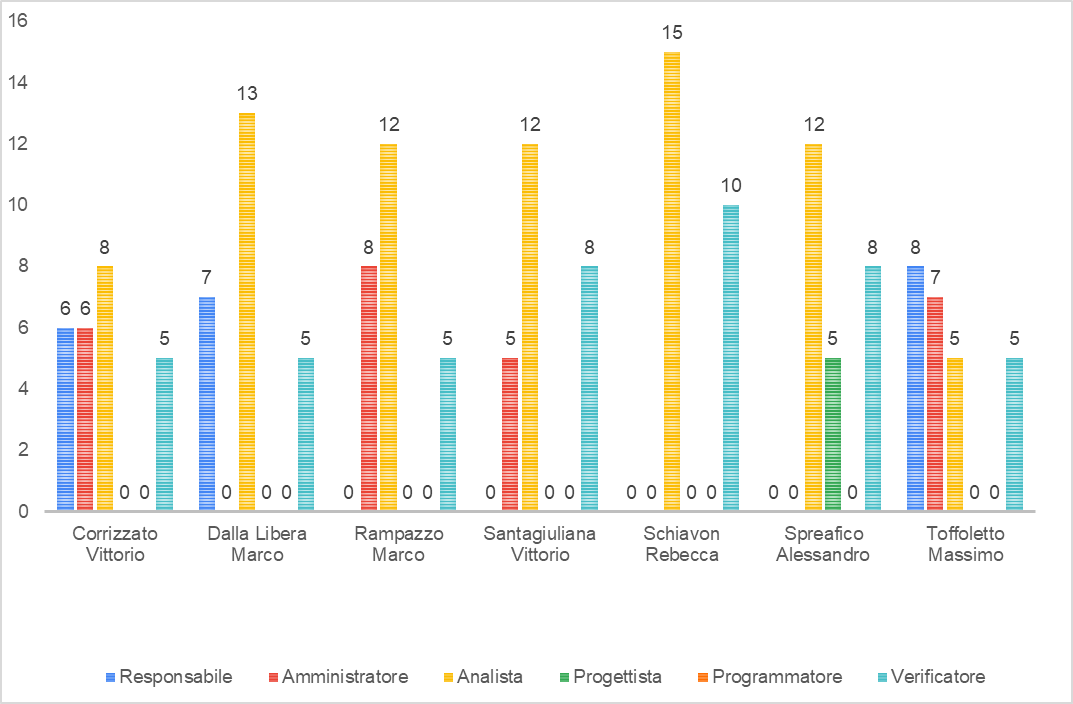
\includegraphics[width=\linewidth]{./img/Grafici/1.png}
	
		\subsubsection{Prospetto economico}
		Nel periodo di analisi sono previsti i seguenti costi:
		\begin{longtable} {
			>{}p{32mm}
			>{}p{20mm}
			>{}p{20mm}
		}
		\rowcolor{gray!50}
		
		\textbf{Ruolo} & \textbf{Ore} & \textbf{Costo} \TBstrut \\
		Responsabile & 20 & 600 \TBstrut \\
		Amministratore & 26 & 520 \TBstrut \\
		Analista & 71 & 1562 \TBstrut \\
		Progettista & 15 & 330 \TBstrut \\
		Programmatore & 0 & 0 \TBstrut \\
		Verificatore & 43 & 645 \TBstrut \\
		\textbf{Totale} & \textbf{175}& \textbf{3657} \TBstrut \\		
		\end{longtable}
		Rappresentati nel seguente grafico: \\
		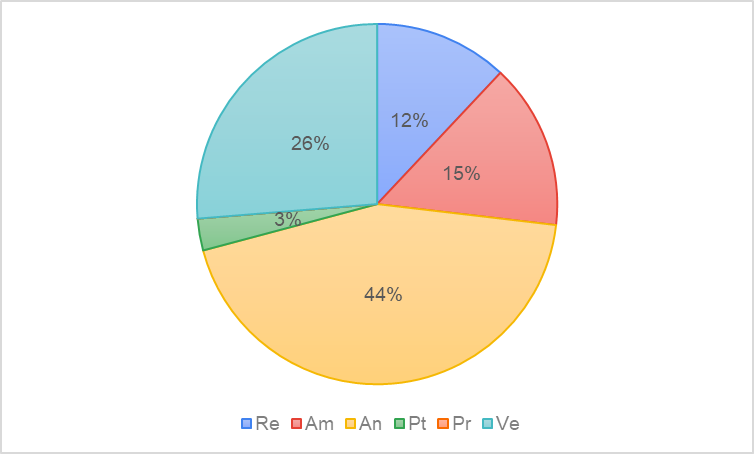
\includegraphics[width=\linewidth]{./img/Grafici/2.png}
\subsection{Periodo di progettazione architetturale}
	\subsubsection{Prospetto orario}
	Nel periodo di analisi è prevista la seguente divisione oraria:
	\begin{longtable} {				
		>{}p{40mm}  
		>{}p{8mm}
		>{}p{8mm}
		>{}p{8mm}
		>{}p{8mm}
		>{}p{8mm}
		>{}p{8mm}
		>{}p{12mm}				
	}			
	\rowcolor{gray!50}
	\textbf{Nominativo} & \textbf{Re} & \textbf{Am} & \textbf{An} & \textbf{Pt} & \textbf{Pr} & \textbf{Ve} & \textbf{Totale}	\TBstrut \\ [2mm]
	Corrizzato Vittorio & - & - & 6 & 10 & 5 & 7 & 28 \TBstrut \\ [2mm]
	Dalla Libera Marco & - & 5 & 7 & - & 7 & 9 & 28 \TBstrut \\ [2mm]
	Rampazzo Marco & 6 & - & - & 9 & 8 & 5 & 28 \TBstrut \\ [2mm]
	Santagiuliana Vittorio & - & - & - & 14 & 5 & 9 & 28 \TBstrut \\ [2mm]
	Schiavon Rebecca & 7 & - & - & - & 9 & 12 & 28 \TBstrut \\ [2mm]
	Spreafico Alessandro & - & 5 & 5 & - & 10 & 8 & 28 \TBstrut \\ [2mm]
	Toffoletto Massimo & - & - & 6 & 5 & 7 & 10 & 28 \TBstrut \\ [2mm]
	\end{longtable}
	Rappresentata nel seguente grafico: \\
	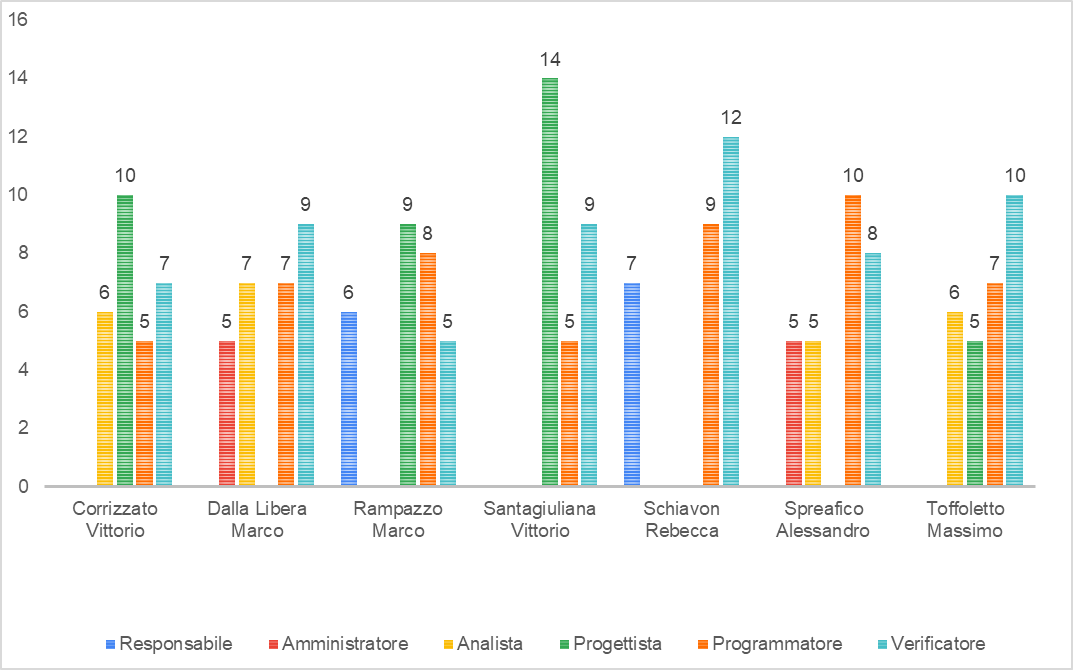
\includegraphics[width=\linewidth]{./img/Grafici/3.png}

\subsubsection{Prospetto economico}
Nel periodo di progettazione architetturale sono previsti i seguenti costi:
\begin{longtable} {
		>{}p{32mm}
		>{}p{20mm}
		>{}p{20mm}
	}
	\rowcolor{gray!50}
	
	\textbf{Ruolo} & \textbf{Ore} & \textbf{Costo} \TBstrut \\
	Responsabile & 13 & 390 \TBstrut \\
	Amministratore & 10 & 200 \TBstrut \\
	Analista & 24 & 528 \TBstrut \\
	Progettista & 38 & 836 \TBstrut \\
	Programmatore & 51 & 765 \TBstrut \\
	Verificatore & 60 & 900 \TBstrut \\
	\textbf{Totale} & \textbf{196}& \textbf{3619} \TBstrut \\		
\end{longtable}	
Rappresentati nel seguente grafico: \\
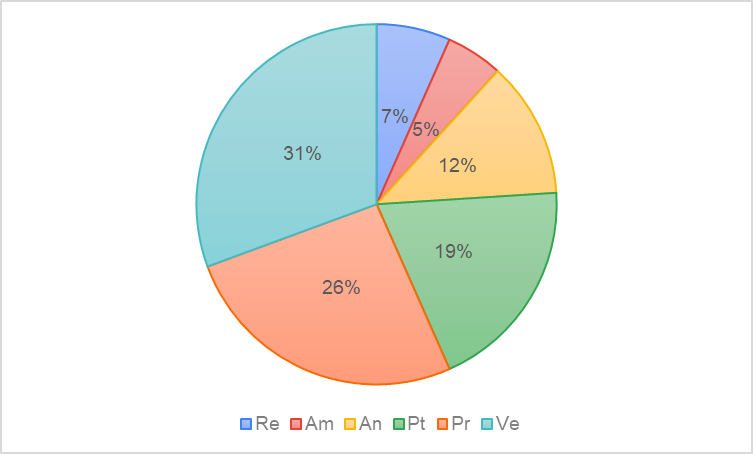
\includegraphics[width=\linewidth]{./img/Grafici/4.png}

\subsection{Periodo di progettazione dettaglio e codifica}
\subsubsection{Prospetto orario}
Nel periodo di progettazione dettaglio e codifica è prevista la seguente divisione oraria:
\begin{longtable} {				
		>{}p{40mm}  
		>{}p{8mm}
		>{}p{8mm}
		>{}p{8mm}
		>{}p{8mm}
		>{}p{8mm}
		>{}p{8mm}
		>{}p{12mm}				
	}			
	\rowcolor{gray!50}
	\textbf{Nominativo} & \textbf{Re} & \textbf{Am} & \textbf{An} & \textbf{Pt} & \textbf{Pr} & \textbf{Ve} & \textbf{Totale}	\TBstrut \\ [2mm]
	Corrizzato Vittorio & - & - & 9 & 23 & 22 & - & 54 \TBstrut \\ [2mm]
	Dalla Libera Marco & 9 & - & 6 & 15 & 15 & 9 & 54 \TBstrut \\ [2mm]
	Rampazzo Marco & - & 5 & - & 23 & 18 & 8 & 54 \TBstrut \\ [2mm]
	Santagiuliana Vittorio & 8 & - & - & 20 & 15 & 11 & 54 \TBstrut \\ [2mm]
	Schiavon Rebecca & - & - & 8 & 20 & 18 & 8 & 54 \TBstrut \\ [2mm]
	Spreafico Alessandro & 8 & - & 0 & 16 & 18 & 12 & 54 \TBstrut \\ [2mm]
	Toffoletto Massimo & - & 5 & - & 23 & 15 & 11 & 54 \TBstrut \\ [2mm]
\end{longtable}
Rappresentata nel seguente grafico: \\
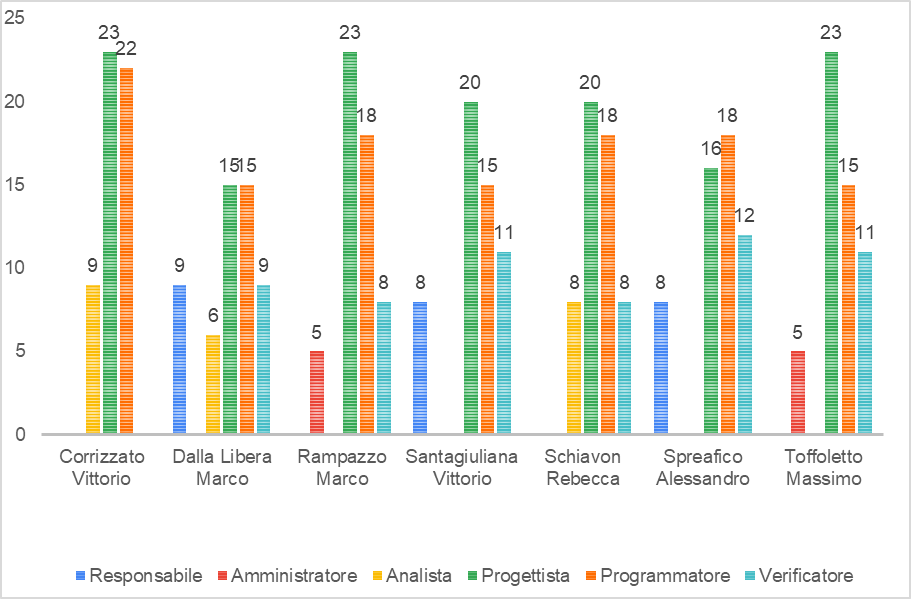
\includegraphics[width=\linewidth]{./img/Grafici/5.png}
\subsubsection{Prospetto economico}
Nel periodo di progettazione dettaglio e codifica sono previsti i seguenti costi:
\begin{longtable} {
		>{}p{32mm}
		>{}p{20mm}
		>{}p{20mm}
	}
	\rowcolor{gray!50}
	
	\textbf{Ruolo} & \textbf{Ore} & \textbf{Costo} \TBstrut \\
	Responsabile & 25 & 750 \TBstrut \\
	Amministratore & 10 & 200 \TBstrut \\
	Analista & 23 & 506 \TBstrut \\
	Progettista & 140 & 3080 \TBstrut \\
	Programmatore & 121 & 1815 \TBstrut \\
	Verificatore & 59 & 885 \TBstrut \\
	\textbf{Totale} & \textbf{378}& \textbf{7236} \TBstrut \\		
\end{longtable}
Rappresentati nel seguente grafico: \\
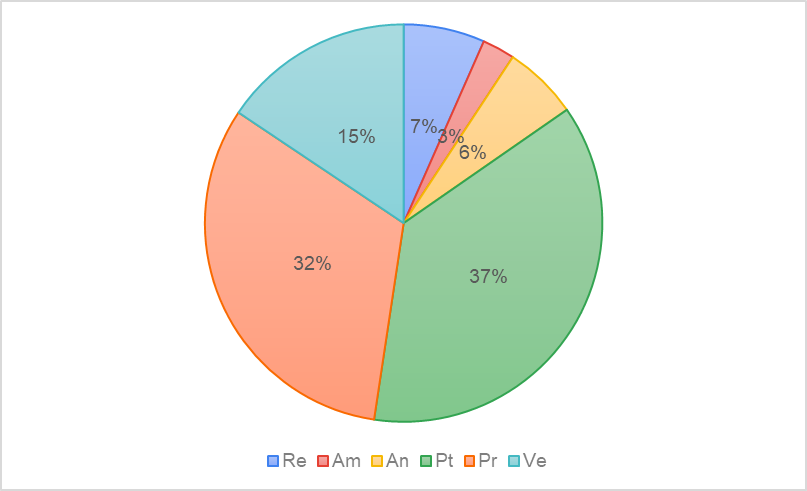
\includegraphics[width=\linewidth]{./img/Grafici/6.png}

\subsection{Periodo di validazione e collaudo}
\subsubsection{Prospetto orario}
Nel periodo di validazione e collaudo è prevista la seguente divisione oraria:
\begin{longtable} {				
		>{}p{40mm}  
		>{}p{8mm}
		>{}p{8mm}
		>{}p{8mm}
		>{}p{8mm}
		>{}p{8mm}
		>{}p{8mm}
		>{}p{12mm}			
	}			
	\rowcolor{gray!50}
	\textbf{Nominativo} & \textbf{Re} & \textbf{Am} & \textbf{An} & \textbf{Pt} & \textbf{Pr} & \textbf{Ve} & \textbf{Totale}	\TBstrut \\ [2mm]
	Corrizzato Vittorio & - & - & - & - & 10 & 10 & 20 \TBstrut \\ [2mm]
	Dalla Libera Marco & 8 & 5 & - & - & 7 & - & 20 \TBstrut \\ [2mm]
	Rampazzo Marco & - & - & - & 5 & 8 & 7 & 20 \TBstrut \\ [2mm]
	Santagiuliana Vittorio & - & 5 & - & - & 6 & 9 & 20 \TBstrut \\ [2mm]
	Schiavon Rebecca & - & 8 & - & - & 7 & 5 & 20 \TBstrut \\ [2mm]
	Spreafico Alessandro & - & - & - & - & 8 & 12 & 20 \TBstrut \\ [2mm]
	Toffoletto Massimo & - & - & - & - & 9 & 11 & 20 \TBstrut \\ [2mm]
\end{longtable}
Rappresentata nel seguente grafico: \\
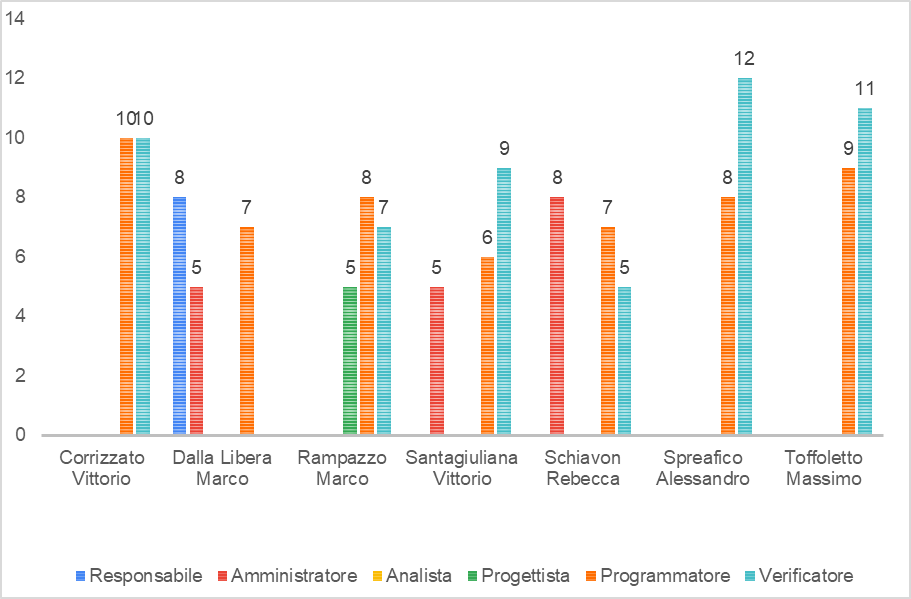
\includegraphics[width=\linewidth]{./img/Grafici/7.png}

\subsubsection{Prospetto economico}
Nel periodo di validazione e collaudo sono previsti i seguenti costi:
\begin{longtable} {
		>{}p{32mm}
		>{}p{20mm}
		>{}p{20mm}
	}
	\rowcolor{gray!50}
	
	\textbf{Ruolo} & \textbf{Ore} & \textbf{Costo} \TBstrut \\
	Responsabile & 8 & 240 \TBstrut \\
	Amministratore & 18 & 360 \TBstrut \\
	Analista & 0 & 0 \TBstrut \\
	Progettista & 5 & 110 \TBstrut \\
	Programmatore & 55 & 825 \TBstrut \\
	Verificatore & 54 & 810 \TBstrut \\
	\textbf{Totale} & \textbf{140}& \textbf{2345} \TBstrut \\		
\end{longtable}
Rappresentati nel seguente grafico: \\
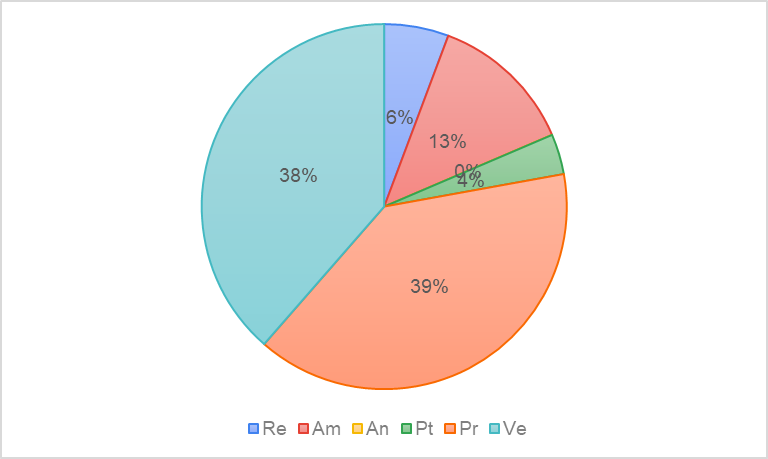
\includegraphics[width=\linewidth]{./img/Grafici/8.png}
	
\section{Consultivi di periodo}
Vengono riportati gli effettivi costi sostenuti per ogni periodo con le eventuali differenze rispetto a quanto preventivato. Il bilancio risulterà quindi:
\begin{itemize}
	\item \textbf{Positivo}: se i costi del consultivo risultano minori di quelli del preventivo;
	\item \textbf{Pari}: se i costi del consultivo risultano uguali a quelli del preventivo;
	\item \textbf{Negativo}: se i costi del consultivo risultano superiori a quelli del preventivo.
\end{itemize}
Seguiranno quindi le conclusioni con le motivazioni delle eventuali differenze e le contromisure che il gruppo ha deciso di attuare per evitare ulteriori discrepanze con quanto dichiarato nel preventivo.

	\subsection{Periodo di Analisi}
	La tabella riporta il numero di ore effettivamente svolte dal gruppo e il rispettivo costo con le eventuali differenze rilevate rispetto al preventivo.
	\begin{longtable} {							
			>{}p{40mm}  
			>{}p{20mm}	
			>{}p{28mm}			
		}			
		\rowcolor{gray!50}
		
		\textbf{Ruolo} & \textbf{Ore} & \textbf{Costo} \TBstrut \\
		Responsabile & 20 & 600 \TBstrut \\
		Amministratore & 25(-1) & 500(-20) \TBstrut \\
		Analista & 80(+9)& 1760(+198) \TBstrut \\
		Progettista & 21(+6) & 462(+132) \TBstrut \\
		Programmatore & 0 & 0 \TBstrut \\
		Verificatore & 43 & 645 \TBstrut \\
		\textbf{Totale Preventivo} & 175 & 3657	\TBstrut \\	
		\textbf{Totale Consultivo} & 189 & 3967	\TBstrut \\	
		\textbf{Differenza Totale} & 14 & 310 	\TBstrut \\	
	\end{longtable}

		\subsubsection{Conclusioni}
		Il bilancio risulta negativo perché le ore effettivamente svolte nei ruoli di analista, progettista e verificatore hanno superato le ore previste dal preventivo.
		Le motivazioni che hanno portato alla necessità di lavorare più del previsto sono le seguenti:
		\begin{itemize}
			\item Analisiti: la stesura dell'\textit{Analisi dei Requisiti} è risultata più complessa del previsto in particolare nell'individuazione dei casi d'uso e dei requisiti;
			\item Progettisti: sono sorte complicazioni non preventivate nella stesura del \textit{Piano di Qualifica} che hanno portato alla necessità di svolgere maggiore attività di autoapprendimento e ad un conseguente rallentamento del lavoro.
		\end{itemize}
		\subsubsection{Preventivo a finire}
		Il periodo di analisi è da intendersi come periodo di investimento per il gruppo e non viene quindi rendicontato, nel budget finale la variazione tra le ore previste e le ore effettive non provocherà alcun cambiamento. 
		È stato inoltre deciso di non modificare i successivi prospetti orari in quanto le condizioni che hanno portato alla necessità di lavorare più di quanto preventivato non dovrebbero presentarsi nuovamente. Il gruppo si ritiene ora più consapevole e meglio preparato, grazie anche alle ore di autoapprendimento già effettuate, e continua a considerare ragionevoli i prospetti orari dei prossimi periodi.


\end{document}